\documentclass[tikz,border=10pt]{standalone}
\usepackage{tikz}
\usetikzlibrary{arrows.meta, positioning, calc, decorations.pathreplacing}
\usepackage{amsmath, amssymb}

% GDL color palette
\definecolor{gdlblue}{RGB}{41, 98, 168}
\definecolor{gdlred}{RGB}{191, 49, 49}
\definecolor{gdlgreen}{RGB}{30, 130, 76}
\definecolor{gdlorange}{RGB}{217, 130, 30}
\definecolor{gdlpurple}{RGB}{118, 56, 138}
\definecolor{gdlgray}{RGB}{140, 140, 140}
\definecolor{gdlyellow}{RGB}{190, 140, 10}

\begin{document}
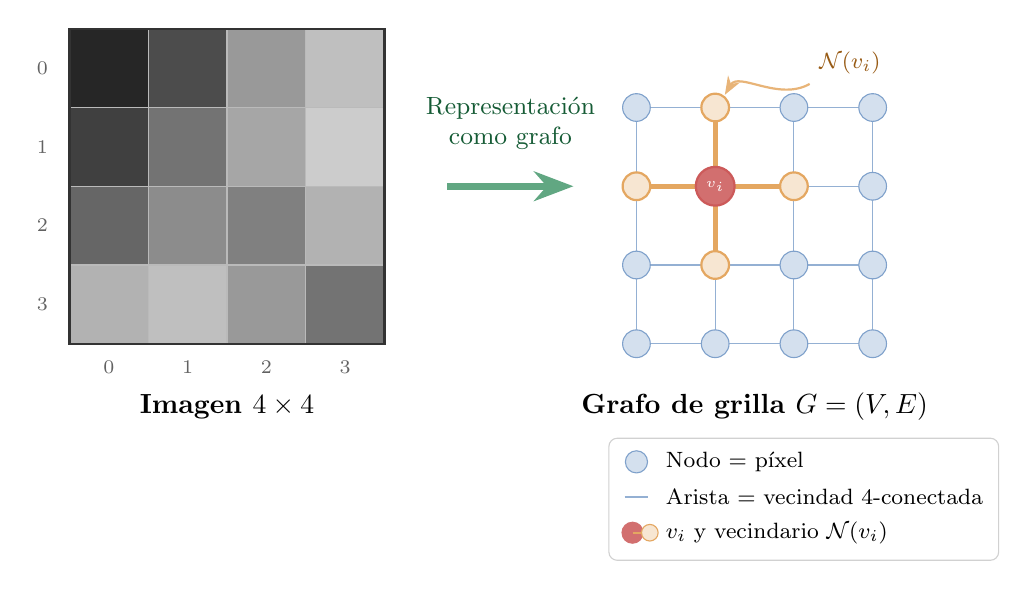
\begin{tikzpicture}[>=Stealth]

% ============================================================
% LEFT PANEL: 4x4 pixel grid (image)
% ============================================================

\def\cs{1.0} % cell size

% Gray values for each pixel: percentage for black!X fill
% Varied intensities to simulate a realistic small image
\def\pixeldata{%
  {85, 70, 40, 25},%  row 0 (top of image)
  {75, 55, 35, 20},%  row 1
  {60, 45, 50, 30},%  row 2
  {30, 25, 40, 55}%   row 3 (bottom of image)
}

% Draw filled cells
\foreach \row [count=\ri from 0] in \pixeldata {
  \foreach \val [count=\ci from 0] in \row {
    \pgfmathsetmacro{\cx}{\ci*\cs + \cs/2}
    \pgfmathsetmacro{\cy}{(3-\ri)*\cs + \cs/2}
    \fill[black!\val] (\cx, \cy) +(-\cs/2,-\cs/2) rectangle +(\cs/2,\cs/2);
    \draw[gdlgray!60, thin] (\cx, \cy) +(-\cs/2,-\cs/2) rectangle +(\cs/2,\cs/2);
  }
}

% Outer border
\draw[black!80, thick] (0, 0) rectangle (4*\cs, 4*\cs);

% Row indices (left side, image convention: 0 at top)
\foreach \r in {0,...,3} {
  \pgfmathsetmacro{\ry}{(3-\r)*\cs + \cs/2}
  \node[font=\scriptsize, text=gdlgray!70!black, left] at (-0.15, \ry) {\r};
}

% Column indices (bottom)
\foreach \c in {0,...,3} {
  \pgfmathsetmacro{\cx}{\c*\cs + \cs/2}
  \node[font=\scriptsize, text=gdlgray!70!black, below] at (\cx, -0.1) {\c};
}

% Label
\node[font=\bfseries, align=center, text=black] at (2*\cs, -0.8)
  {Imagen $4 \times 4$};

% ============================================================
% ARROW
% ============================================================

\draw[->, gdlgreen!70, line width=2.5pt] (4.8, 2.0) -- (6.4, 2.0);
\node[font=\small, align=center, text=gdlgreen!70!black] at (5.6, 2.8)
  {Representaci\'{o}n\\como grafo};

% ============================================================
% RIGHT PANEL: Graph grid with 4-connectivity
% ============================================================

\def\gs{1.0}    % grid spacing
\def\nsize{5pt} % node radius

% Origin for graph grid
\def\gox{7.2}
\def\goy{0.0}

% Highlighted node: col=1, row=2 (0-indexed from bottom-left in TikZ coords)
% This corresponds to image pixel (row=1, col=1)
\def\hcol{1}
\def\hrow{2}

% --- Draw regular edges (4-connectivity) ---
\foreach \r in {0,...,3} {
  \foreach \c in {0,...,3} {
    % Horizontal edge to the right
    \pgfmathtruncatemacro{\cnext}{\c+1}
    \ifnum\cnext<4
      \pgfmathtruncatemacro{\isHighEdgeH}{%
        (\r==\hrow && \c==\hcol) ||
        (\r==\hrow && \cnext==\hcol) ? 1 : 0}
      \ifnum\isHighEdgeH=0
        \draw[gdlblue!50] (\gox+\c*\gs, \goy+\r*\gs) -- (\gox+\cnext*\gs, \goy+\r*\gs);
      \fi
    \fi
    % Vertical edge upward
    \pgfmathtruncatemacro{\rnext}{\r+1}
    \ifnum\rnext<4
      \pgfmathtruncatemacro{\isHighEdgeV}{%
        (\c==\hcol && \r==\hrow) ||
        (\c==\hcol && \rnext==\hrow) ? 1 : 0}
      \ifnum\isHighEdgeV=0
        \draw[gdlblue!50] (\gox+\c*\gs, \goy+\r*\gs) -- (\gox+\c*\gs, \goy+\rnext*\gs);
      \fi
    \fi
  }
}

% --- Draw highlighted edges (center node to its 4 neighbors) ---
\draw[gdlorange!70, line width=1.8pt]
  (\gox+\hcol*\gs, \goy+\hrow*\gs) -- (\gox+2*\gs, \goy+2*\gs);
\draw[gdlorange!70, line width=1.8pt]
  (\gox+\hcol*\gs, \goy+\hrow*\gs) -- (\gox+0*\gs, \goy+2*\gs);
\draw[gdlorange!70, line width=1.8pt]
  (\gox+\hcol*\gs, \goy+\hrow*\gs) -- (\gox+1*\gs, \goy+3*\gs);
\draw[gdlorange!70, line width=1.8pt]
  (\gox+\hcol*\gs, \goy+\hrow*\gs) -- (\gox+1*\gs, \goy+1*\gs);

% --- Draw nodes ---
\foreach \r in {0,...,3} {
  \foreach \c in {0,...,3} {
    \pgfmathtruncatemacro{\iscenter}{(\r==\hrow && \c==\hcol) ? 1 : 0}
    \pgfmathtruncatemacro{\isneighbor}{%
      ((\r==\hrow && \c==\hcol+1) ||
       (\r==\hrow && \c==\hcol-1) ||
       (\c==\hcol && \r==\hrow+1) ||
       (\c==\hcol && \r==\hrow-1)) ? 1 : 0}
    \ifnum\iscenter=1
      % Center node (red, larger)
      \fill[gdlred!70] (\gox+\c*\gs, \goy+\r*\gs) circle (7pt);
      \draw[gdlred!80, thick] (\gox+\c*\gs, \goy+\r*\gs) circle (7pt);
      \node[font=\tiny\bfseries, text=white] at (\gox+\c*\gs, \goy+\r*\gs) {$v_i$};
    \else
      \ifnum\isneighbor=1
        % Neighbor nodes (orange outline)
        \fill[gdlorange!20] (\gox+\c*\gs, \goy+\r*\gs) circle (\nsize);
        \draw[gdlorange!70, thick] (\gox+\c*\gs, \goy+\r*\gs) circle (\nsize);
      \else
        % Regular nodes (blue)
        \fill[gdlblue!20] (\gox+\c*\gs, \goy+\r*\gs) circle (\nsize);
        \draw[gdlblue!60] (\gox+\c*\gs, \goy+\r*\gs) circle (\nsize);
      \fi
    \fi
  }
}

% --- Neighborhood annotation ---
% Arrow from label to one of the neighbor nodes (top neighbor at (1,3))
\node[font=\footnotesize, text=gdlorange!70!black, anchor=south west]
  (Nlabel) at (\gox+2.2*\gs, \goy+3.3*\gs) {$\mathcal{N}(v_i)$};
\draw[->, gdlorange!60, thick, shorten >=3pt]
  (Nlabel.south west) to[out=-150, in=60] (\gox+\hcol*\gs+0.07, \goy+3*\gs+0.07);

% Label
\node[font=\bfseries, align=center, text=black] at (\gox+1.5*\gs, -0.8)
  {Grafo de grilla $G = (V, E)$};

% ============================================================
% LEGEND (below the graph panel)
% ============================================================

\def\lx{7.2}
\def\ly{-1.5}

% Background box for legend
\fill[white, draw=gdlgray!40, rounded corners=3pt]
  (\lx-0.35, \ly-1.25) rectangle (\lx+4.6, \ly+0.3);

% Node = pixel
\fill[gdlblue!20] (\lx, \ly) circle (4pt);
\draw[gdlblue!60] (\lx, \ly) circle (4pt);
\node[font=\footnotesize, text=black, anchor=west] at (\lx+0.25, \ly)
  {Nodo $=$ p\'{i}xel};

% Edge = 4-connected neighborhood
\draw[gdlblue!50, thick] (\lx-0.15, \ly-0.45) -- (\lx+0.15, \ly-0.45);
\node[font=\footnotesize, text=black, anchor=west] at (\lx+0.25, \ly-0.45)
  {Arista $=$ vecindad 4-conectada};

% Highlighted neighborhood
\fill[gdlred!70] (\lx-0.05, \ly-0.9) circle (4pt);
\draw[gdlorange!70, thick] (\lx-0.05, \ly-0.9) -- (\lx+0.17, \ly-0.9);
\fill[gdlorange!20] (\lx+0.17, \ly-0.9) circle (3pt);
\draw[gdlorange!70] (\lx+0.17, \ly-0.9) circle (3pt);
\node[font=\footnotesize, text=black, anchor=west] at (\lx+0.25, \ly-0.9)
  {$v_i$ y vecindario $\mathcal{N}(v_i)$};

\end{tikzpicture}
\end{document}
